\documentclass[12pt]{article}

\usepackage{sbc-template}

\usepackage{graphicx,url}

%\usepackage[brazil]{babel}   
\usepackage[latin1]{inputenc}  

\usepackage{amsmath}
\usepackage{amssymb} 
\usepackage{mathtools}

\usepackage{algorithm}
\usepackage[noend]{algpseudocode}

\usepackage{hyperref}
 
\newcommand{\Cfield}{\mathbb{C}}
\newcommand{\Rfield}{\mathbb{R}}

\newcommand{\norm}[1]{\left\lVert#1\right\rVert}

\sloppy

\title{PCS5120 Homework}

\author{Giuliano A. F. Belinassi\inst{1}}


\address{Institute of Mathematics and Statistics (IME) -- University of S�o Paulo
  (USP)\\
  Rua do Mat�o, 1010 -- S�o Paulo -- SP -- Brazil
}

\begin{document} 

\maketitle

%\begin{abstract}

%The Boundary Element Method requires a geometry discretization to execute simulations, 
%and it can be used to analyze the 3D stationary behavior of wave propagation in the soil. 
%Such discretization involves generating two high computational power demanding matrices, 
%and this article demonstrates how Graphical Processing Units (GPU) were used to accelerate 
%this process. In an experiment with 4000 Mesh elements and 1600 Boundary elements, 
%a speedup of 107$\times$ was obtained with a GeForce GTX980. 

%\end{abstract}
     
%\section{Introduction}

In various research fields where computational linear algebra is required eighter because of 
its facility or inexisence of analytical solutions, can take advantage of numerical linear 
algebra packages such as Lapack or BLAS. One major concern about these libraries is its 
performance, subject discussed in this report. Here we target the routine designed to multiply 
two matrices in single precision floating point (\texttt{SGEMM}).

Althrough implementing a matrix-matrix multiplication seems trivial by its concept, it is 
fairly difficult to provide an efficient code because of various reasons, such as cache usage. 
The use of techniques such as block matrix-matrix multiplication can yield better results due 
to a better cache usage, but a question that can be asked from this approach is what is the 
block size that maximizes performance?


\section{The database}

We used the database "\textit{SGEMM GPU kernel performance Data Set}" provided by \textit{UCI machine 
learning repository}\footnote{\url{https://archive.ics.uci.edu/ml/datasets/SGEMM+GPU+kernel+performance}}. 
Briefly, it has timings of multiplication of two matrices in \textit{ms}, each 
one of size $2048\times2048$, using a combination of $14$ parameters, totalizing $241601$ lines in the database. 
Since the database provides four run times per line, we added a new column "mean" that is the average of these values.

\section{Data analysis}

We used Orange in our analysis. Our first objective was to find the distribuition of the average 
of the four executions per sample to check possible improvements or deterioration of the performance. 
Figure \ref{fig:freq} shows such distribution. Notice that most of the averages concentrate under 200ms, 
and there are some data aroung 2400ms. Such high timing can be caused by the parameters itself or be an 
outlier because there were other programs running on the computer.

\begin{figure}[ht]
\centering
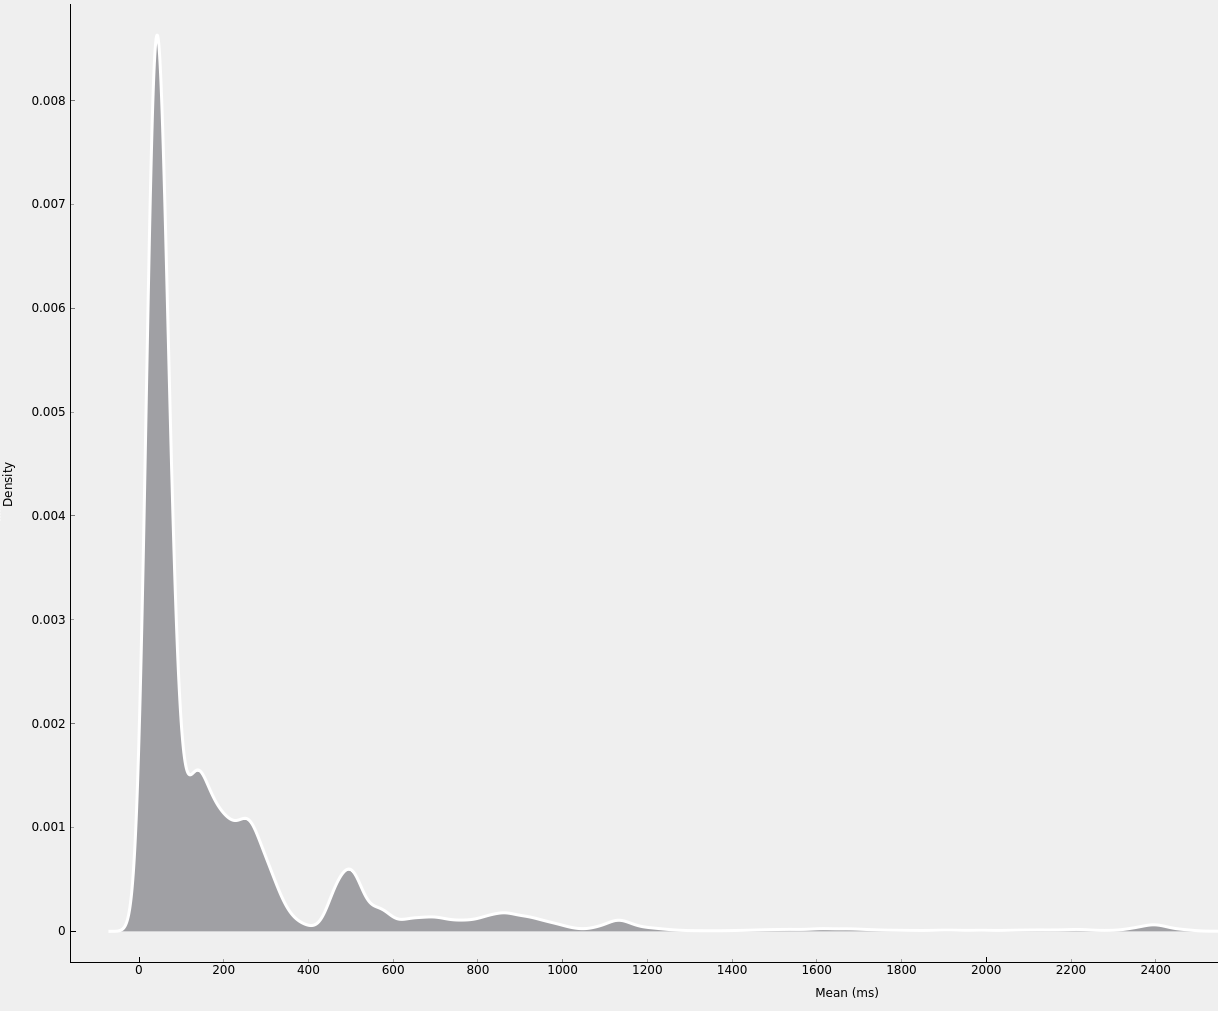
\includegraphics[scale=0.35]{freq.png}
\caption{Distribution of the average of four samples per parameter.}
\label{fig:freq}
\end{figure}

\section{Conclusions}


%The current implemented code have limitations. First, there is no logic to construct both $H$ and $G$ by blocks to create several 
%GPU kernels. Second, there is also no logic to compute both $\texttt{Ghmatecd\_Nonsingd}$ and $\texttt{Ghmatecd\_Sing\_de}$ in 
%parallel with respect to each other. The usage of GPUs in the singular case can also be analyzed.


%\begin{figure}[ht]
%\centering
%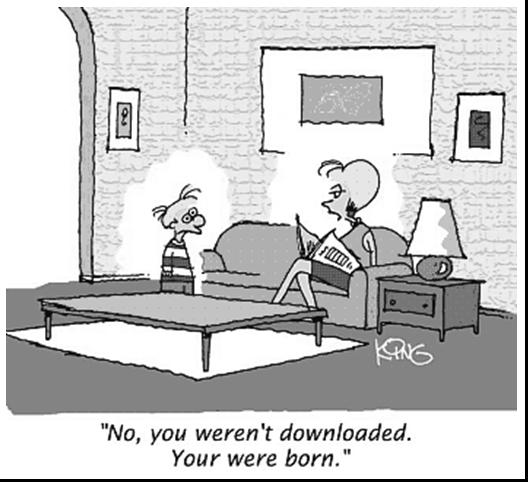
\includegraphics[width=.5\textwidth]{fig1.jpg}
%\caption{A typical figure}
%\label{fig:exampleFig1}
%\end{figure}
%
%\begin{figure}[ht]
%\centering
%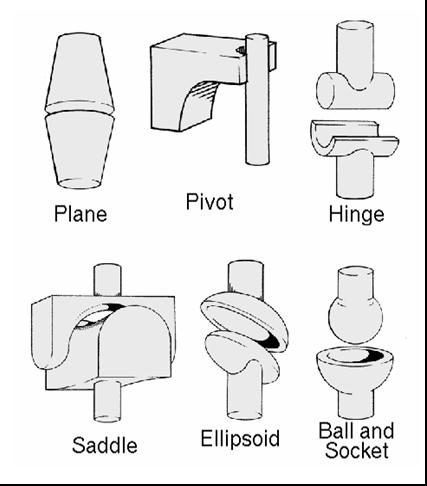
\includegraphics[width=.3\textwidth]{fig2.jpg}
%\caption{This figure is an example of a figure caption taking more than one
%  line and justified considering margins mentioned in Section~\ref{sec:figs}.}
%\label{fig:exampleFig2}
%\end{figure}


\bibliographystyle{sbc}
\bibliography{sbc-template}

\end{document}
\grid
